%!TEX root = ../../dimensions-2016-game-book.tex


\phWorksheet{The Math Behind the Puzzle}

  The Main Puzzle was inspired by the Mutilated Chessboard problem, first posed
  by Max Black in his book \textit{Critical Thinking} (1946), and often
  associated with famous mathematical puzzler Martin Gardner who considered
  it in his \textit{Mathematical Games} column in \textit{Scientific American}.
  The problem asks if a chessboard missing its corners \(a1,h8\)
  may be tiled by dominoes.

  \begin{center}
    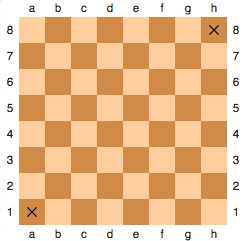
\includegraphics[width=0.3\linewidth]{mutilated-chessboard.png}
  \end{center}

  The solution boils down to the fact that any domino must cover exactly one
  cell of each color, black and white. This same technique may be extended
  to identify impossible letters in Domino Rally.

  \begin{center}
  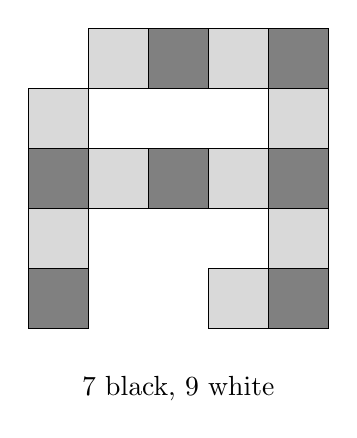
\begin{tikzpicture}[x=0.3in,y=0.3in]
    \draw[fill=gray]  (0,0) rectangle +(1,1);
    \draw[fill=white!70!gray] (0,1) rectangle +(1,1);
    \draw[fill=gray]  (0,2) rectangle +(1,1);
    \draw[fill=white!70!gray] (0,3) rectangle +(1,1);

    \draw[fill=white!70!gray] (1,2) rectangle +(1,1);
    \draw[fill=gray]  (2,2) rectangle +(1,1);
    \draw[fill=white!70!gray] (3,2) rectangle +(1,1);

    \draw[fill=white!70!gray] (1,4) rectangle +(1,1);
    \draw[fill=gray]  (2,4) rectangle +(1,1);
    \draw[fill=white!70!gray] (3,4) rectangle +(1,1);
    \draw[fill=gray]  (4,4) rectangle +(1,1);

    \draw[fill=white!70!gray] (4,3) rectangle +(1,1);
    \draw[fill=gray]  (4,2) rectangle +(1,1);
    \draw[fill=white!70!gray] (4,1) rectangle +(1,1);
    \draw[fill=gray]  (4,0) rectangle +(1,1);
    \draw[fill=white!70!gray] (3,0) rectangle +(1,1);

    \node at (2.5,-1) {7 black, 9 white};
  \end{tikzpicture}
  \hspace{0.5in}
  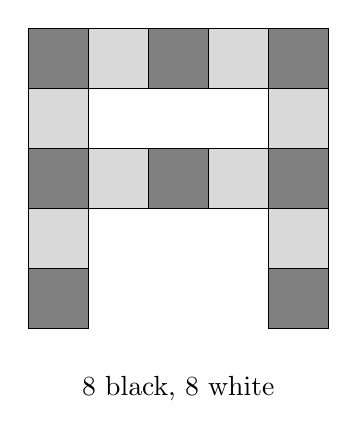
\begin{tikzpicture}[x=0.3in,y=0.3in]
    \draw[fill=gray]  (0,0) rectangle +(1,1);
    \draw[fill=white!70!gray] (0,1) rectangle +(1,1);
    \draw[fill=gray]  (0,2) rectangle +(1,1);
    \draw[fill=white!70!gray] (0,3) rectangle +(1,1);
    \draw[fill=gray]  (0,4) rectangle +(1,1);

    \draw[fill=white!70!gray] (1,2) rectangle +(1,1);
    \draw[fill=gray]  (2,2) rectangle +(1,1);
    \draw[fill=white!70!gray] (3,2) rectangle +(1,1);

    \draw[fill=white!70!gray] (1,4) rectangle +(1,1);
    \draw[fill=gray]  (2,4) rectangle +(1,1);
    \draw[fill=white!70!gray] (3,4) rectangle +(1,1);
    \draw[fill=gray]  (4,4) rectangle +(1,1);

    \draw[fill=white!70!gray] (4,3) rectangle +(1,1);
    \draw[fill=gray]  (4,2) rectangle +(1,1);
    \draw[fill=white!70!gray] (4,1) rectangle +(1,1);
    \draw[fill=gray]  (4,0) rectangle +(1,1);

    \node at (2.5,-1) {8 black, 8 white};
  \end{tikzpicture}
  \end{center}

  An equal number of black and white squares in a letter doesn't guarantee a
  tiling exists, but \textbf{Gomory's theorem} (1974) demonstrates that the
  removal of two opposite colored squares from a chessboard allows for a tiling.